
\chapter{Reconnaissance basée sur l'extraction de \nfw{features}}




Si l'utilisation des données brutes comme entrée des réseaux de neurones 
permet déjà d'obtenir des résultats encourageant, il est possible de faire 
mieux en effectuant un pré-traitement des données. 
Il s'agit d'extraire des données brutes (i.e.\/ les pixels de l'image) des 
caractéristiques (ou \nfw{features} en anglais) qui permettent de décrire 
l'image dans un format plus adapté pour une machine.

\newcommand{\features}{\nfw{features}}
Ces \features peuvent être regroupés en deux catégories : 
\begin{enumerate}
  \item les \features statistiques, qui vont s'intéresser à des densité de pixels, 
  des extremums et autres transformées mathématiques;
  \item les \features structurelles, qui s’intéressent aux traits (strokes), aux courbes,
  aux nombres de bifurcations, etc…, ces dernières sont plus intuitives pour l’humain.
\end{enumerate}

Nous allons dans ce chapitre présenter quelques \features qui peuvent être 
utilisées dans le cadre de la reconnaissance de caractères. Puis nous les utiliserons 
comme entrées de différents algorithmes de \nfw{machine learning}.



\section{Binarisation de l'image}



Les images du jeu de données sont en niveaux de gris. 
C'est à dire que chaque pixel est représenté par un entier entre 0 
et 255 (du blanc au noir). 
Certains algorithmes ne prennent pas en compte le niveau de coloration 
du pixel et s'intéresse juste au fait que le pixel soit noir ou blanc. 
Il est donc utile, dans ce cas de binariser l'image (i.e.\/ de passer 
à la convention 0 pour un pixel ne contenant pas d'encre et 1 pour 
un pixel en contenant). 
On choisit donc arbitrairement un seuil à partir duquel on considère que 
le pixel est colorié.

\begin{codeblock}
def binarize(img, treshold = 200):
    w = len(img)
    h = len(img[0])
    ret = img.copy()
    for x in range(w):
        for y in range(h):
            ret[y][x] = 1 if img[y][x] >= treshold else 0
    return ret
\end{codeblock}

Bien évidemment, le choix du seuil peut avoir un impact sur le calcul des 
\features si l'on choisit un seuil très élevé, beaucoup de pixels seront 
considérés comme vide. A contrario, si le seuil est très faible, on considéra 
qu'un pixel est colorié dès qu'il y aura un peu d'encre dessus, ce qui peut 
également poser des problèmes.



\section{Densités de pixels coloriés}



\section{Nombre de croissements (\nfw{crossings})}



On prend deux points à l’extrémité de l’image et on compte le nombre d’alternance 
entre les groupes de pixels vides et les groupes de pixels contenant de l’encre. 
Cette méthode n’est à priori pas sensible à l’épaisseur du trait.



\section{Histogramme des projections}



On compte pour chaque ligne (resp. chaque colonne) le nombre de pixels allumés sur 
la ligne (resp. colonne). 
En faisant ça sur l’ensemble de l’image, on obtient deux histogrammes. 
Cette technique peut aussi être utilisé pour segmenter des lignes et caractères isolés. 
Cette technique peut être sensible à l’épaisseur du trait. 
Pour palier ce problème, on peut renormaliser chaque histogramme en divisant 
chaque valeur par le total.

\begin{figure}[h]
  \centering
  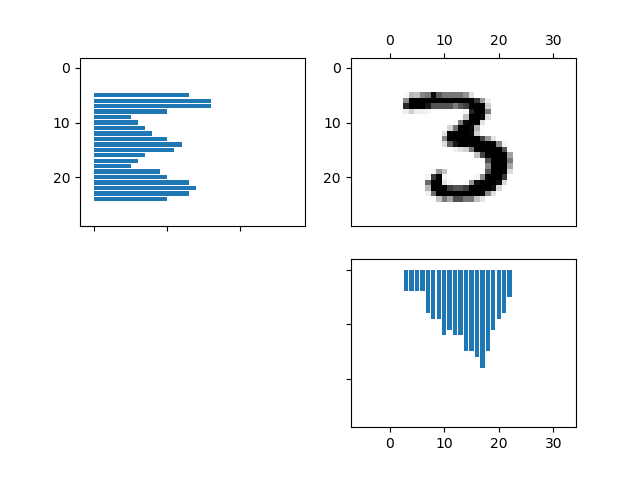
\includegraphics[scale=0.5]{assets/features-hvhisto-ex1}
  \caption{Histogramme des projections du chiffre 3.}
  \label{fig:features-hvhisto-ex1}
\end{figure}



\section{Moments}



Dans tout ce qui suit, on note $p_{xy}$ la valeur du pixel $(x,y)$.

On définit le moment d'ordre $(p+q)$ par:
\[
m_{pq} = \sum_x \sum_y x^p y^q p_{xy}
\]

En pratique, on préférera utiliser des moments centrés (car invariant 
par translation de l'image).
\[
\mu_{pq} = \sum_x \sum_y (x - \overline{x})^p (y - \overline{y})^q p_{xy}
\]
avec 
\[
\overline{x} = \frac{m_{10}}{m_{00}} \qquad \qquad \overline{y} = \frac{m_{01}}{m_{00}}
\]



\section{Transformée de Fourier du contour}

On s'intéresse ici au contour des chiffres. 
On peut voir le contour comme une fonction périofique 
de $\mathbb{R}$ dans $\mathbb{R}^2$. 
On peut donc lui appliquer une transformée de Fourier pour 
en récupérer un spectre de fréquence. 
En conservant les plus faibles fréquences, on s'intéressera à 
la forme générale du contour sans considérer les détails.

En pratique, on travaille avec un contour discret. 
Dans notre cas, ce contour est stocké en utilisant le codage 
de chaînes de Freeman.
Il s'agit simplement d'un codage indiquant les directions à suivre 
pour tracer le contour (e.g.\/ nord, sub, nord-est, etc...).
Si l'on ajoute à cela un point de départ, on est en mesure de 
reconstruire le contour à partir de la chaîne.

\begin{figure}[h!]
    \centering
    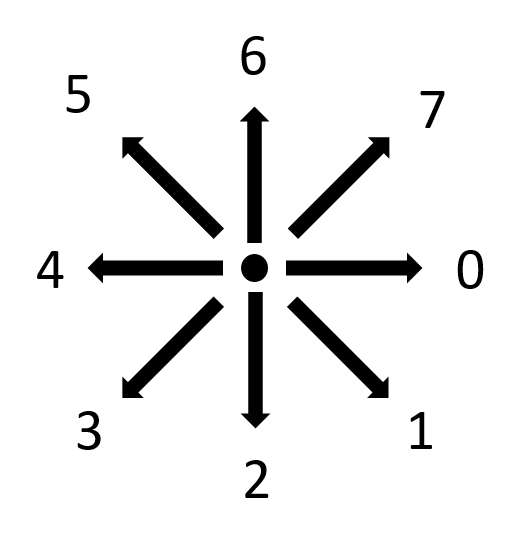
\includegraphics[scale=0.45]{assets/freeman-chain-encoding}
    \caption{Codage de Freeman d'une chaîne.}
	\label{fig:freeman-chain-encoding}
\end{figure}

On code donc un contour comme un $K$-uplet $a_1, \cdots a_K$ 
où les $a_i$ sont des entiers dans $\llbracket 0, 7 \rrbracket$. 
On notera $V = a_1 a_2 \cdots a_K$ la chaîne représentant le 
contour.

Cette chaîne définie un ensemble de points $(p_i)_i$ 
dont les coordonnées sont tous des entiers et vérifiant:
\[
\vecnorm{p_i - p_{i-1}} =
\begin{cases}
  1 \text{ si } a_i \text{ est paire;} \\
  \sqrt{2} \text{ sinon;} \\
\end{cases}
\]
avec $p_0 = (0,0)$.

On associe également, pour tout couple de points consécutifs 
un temps de traversé $\Delta t$ qui est égal à la distance 
séparant les deux points.
Cette quantité vérifie donc:
\[
\Delta t_i = 1 + \left( \frac{\sqrt(2) - 1}{2} \right) \left( 1 - (-1)^{a_i} \right)
\]

Le temps mis pour traverser les $p$ premiers liens de la chaîne vaut donc 
\[
t_p = \sum_{i = 1}^{p} \Delta t_i
\]
et la période de la chaîne est $T = t_K$.


Nous avons implémenté une fonction permettant de calculer le 
contour d'une image.
Voici en quelques mots son principe de fonctionnement. 
On commence par partir du pixel situé en haut à droite de l'image 
et on parcours les pixels de gauche à droite et de haut an bas 
jusqu'à trouver un pixel colorié. 
On prend comme point de départ le dernier pixel non colorié sur lequel 
on est passé.
On simule ensuite le comportement d'une coccinelle qui serait posée sur 
sur ce pixel et qui serait orientée direction nord-ouest. 
Le but de la coccinelle est d'avancer en maintenant toujours à sa 
droite les pixels coloriés. 
Pour avancer, elle regarde, à partir de sa direction actuelle, quelle 
est la case la plus à droite qu'elle peut atteindre sans faire demi-tour.
Si la première case à droite qu'elle peut atteindre correspond à un demi-tour, 
elle regarde la première case à sa gauche qu'elle peut atteindre.
[Note: il y a quelques autres subtilités non décrites ici pour simplifier, 
le code est disponible dans le fichier \tcode{features.py}]
L'algorithme se termine quand la coccinelle revient à son point de départ.

\begin{figure}[h!]
    \centering
    \begin{subfigure}[b]{0.4\textwidth}
        \centering
        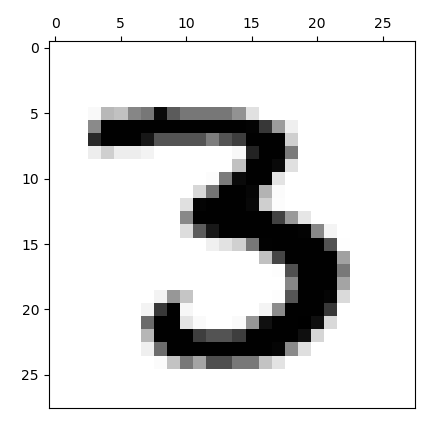
\includegraphics[scale=0.45]{assets/training-image-12}
    \end{subfigure}%
    ~ 
    \begin{subfigure}[b]{0.4\textwidth}
        \centering
        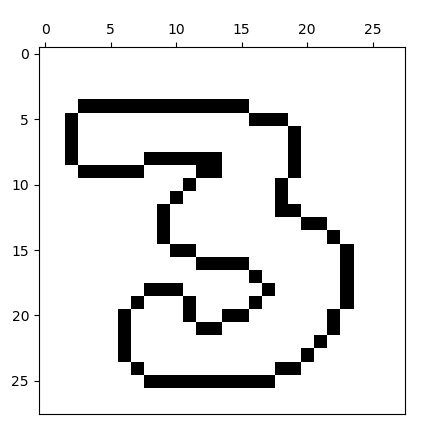
\includegraphics[scale=0.45]{assets/training-image-12-contour}
    \end{subfigure}
    \caption{Contour calculé du chiffre 3.}
\end{figure}

On peut ensuite appliquer une transformée de Fourier à ce contour 
discret. 
Considérons que notre contour est une fonction périodique de 
période $T$ de $\mathbb{R}$ dans $\mathbb{R}^2$ dont les composantes 
sont $x(t)$ et $y(t)$.
Alors sa décomposition en séries de Fourier s'écrit
\[
x(t) = A_0 + \sum_{n = 1}^{+\infty} a_n \cos\left(\frac{2n\pi t}{T}\right) 
  + b_n \sin\left(\frac{2n\pi t}{T}\right) 
\]
où
\[
A_0 = \frac{1}{T} \int_{0}^{T} x(t) \mathrm{d}t  \qquad
a_n = \frac{2}{T} \int_{0}^{T} x(t) \cos\left(\frac{2n\pi t}{T}\right)  \mathrm{d}t  \qquad
b_n = \frac{2}{T} \int_{0}^{T} x(t) \sin\left(\frac{2n\pi t}{T}\right)  \mathrm{d}t 
\]

Nous allons calculer ces coefficients de manière explicite en écrivant 
la dérivée $x'(t)$ de deux manières.
On rappelle que $x$ est dérivable en tout point $t \in ]0, T[$ 
n'appartenant pas à $\{ t_1, \cdots, t_K \}$.

La première écriture s'obtient en appliquant une transformée de Fourier 
à $x'$ qui est une fonction périodique de période $T$. 
\[
x'(t) = \sum_{n = 1}^{+\infty} \alpha_n \cos\left(\frac{2n\pi t}{T}\right) 
  + \beta_n \sin\left(\frac{2n\pi t}{T}\right) 
\]
où
\[
\alpha_n = \frac{2}{T} \int_{0}^{T} x'(t) \cos\left(\frac{2n\pi t}{T}\right)  \mathrm{d}t  \qquad \qquad
\beta_n = \frac{2}{T} \int_{0}^{T} x'(t) \sin\left(\frac{2n\pi t}{T}\right)  \mathrm{d}t 
\]
Il n'y a évidemment pas de terme constant dans cette écriture car 
l'intégrale de $x'$ sur une période vaut 0 puisque $x(0) = x(T)$.

Ces quantités sont faciles à calculer car $x'$ est constante par 
morceaux.
\[
x'(t) = \frac{\Delta x_p}{\Delta t_p} \text{ pour } t_{p-1} < t < t_p
\]

On obtient donc
\begin{align*}
\alpha_n &= \frac{2}{T} \sum_{p = 1}^{K} \frac{\Delta x_p}{\Delta t_p} \int_{t_{p-1}}^{t_p} \cos\left(\frac{2n\pi t}{T}\right)  \mathrm{d}t  \\
         &= \frac{1}{n \pi} \sum_{p = 1}^{K} \frac{\Delta x_p}{\Delta t_p} \left( \sin\left(\frac{2n\pi t_p}{T}\right) - \sin\left(\frac{2n\pi t_{p-1}}{T}\right)  \right)
\end{align*}
De même, 
\[
\beta_n = -\frac{1}{n \pi} \sum_{p = 1}^{K} \frac{\Delta x_p}{\Delta t_p} \left( \cos\left(\frac{2n\pi t_p}{T}\right) - \cos\left(\frac{2n\pi t_{p-1}}{T}\right)  \right)
\]

La seconde expression de $x'(t)$ est obtenue en dérivant directement son 
expression sous forme de série.
\[
x'(t) = \frac{2n\pi}{T}\sum_{n = 1}^{+\infty} -a_n \sin\left(\frac{2n\pi t}{T}\right) 
  + b_n \cos\left(\frac{2n\pi t}{T}\right) 
\]

On écrit ensuite l'égalité des coefficients devant les sinus et cosinus 
d'une période donnée.
\[
\begin{cases}
  \alpha_n = \frac{2n\pi}{T} b_n \\
  \beta_n = \frac{2n\pi}{T} a_n
\end{cases}
\]
Au final, 
\[
a_n = \frac{T}{2 n^2 \pi^2} \sum_{p = 1}^{K} \frac{\Delta x_p}{\Delta t_p} \left[ \cos\left(\frac{2n\pi t_p}{T}\right) - \cos\left(\frac{2n\pi t_{p-1}}{T}\right) \right]
\]
\[
b_n = \frac{T}{2 n^2 \pi^2} \sum_{p = 1}^{K} \frac{\Delta x_p}{\Delta t_p} \left[ \sin\left(\frac{2n\pi t_p}{T}\right) - \sin\left(\frac{2n\pi t_{p-1}}{T}\right) \right]
\]

On peut appliquer le même raisonnement pour $y(t)$ et on obtiendra des 
coefficients $C_0$, $c_n$ et $d_n$ vérifiant les mêmes équations.

On pourra utiliser les coefficients $a_n, b_n, c_n, d_n$ comme 
\nfw{features}.

La figure \ref{fig:contour-reconstruction} montre la reconstruction 
du contour de l'exemple précédent en ajoutant à chaque étape des 
composantes (on commence à l'ordre 1 pour finir à l'ordre 12). 

\begin{figure}[h!]
  \centering
  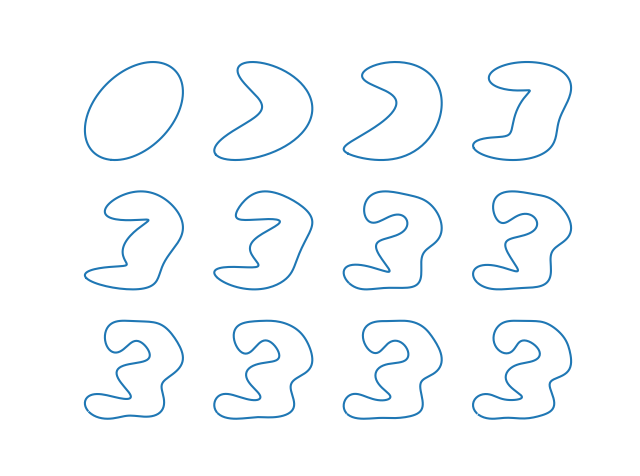
\includegraphics[scale=0.8]{assets/fourier-contour-image12-reconstruction}
  \caption{Reconstruction d'un contour.}
  \label{fig:contour-reconstruction}
\end{figure}

Cette figure permet d'estimer un intervalle d'ordres que l'on pourrait 
utiliser comme \nfw{feature}.



\section{Transformée de Fourier de l'image}

On utilise la fonction \tcode{rfft} de la bibliothèque \tcode{scipy.fftpack} sur 
l'image en niveaux de gris pour passer dans le domaine de Fourier.
La procédure, qui consiste en une double appel à \tcode{rfft}, renvoie une image 
de même taille que l'entrée.

L'image dans le domaine de Fourier est la décomposition de l'image dans le domaine 
fréquentiel.
Il est possible de reconstruire l'image en utilisant la 
fonction \tcode{irfft} de la même bibliothèque.
Cette fonction permet également de visualiser la base utilisée dans le domaine 
fréquentiel (c.f.\/ figure \ref{fig:freq-basis}).

\begin{figure}[h]
  \centering
  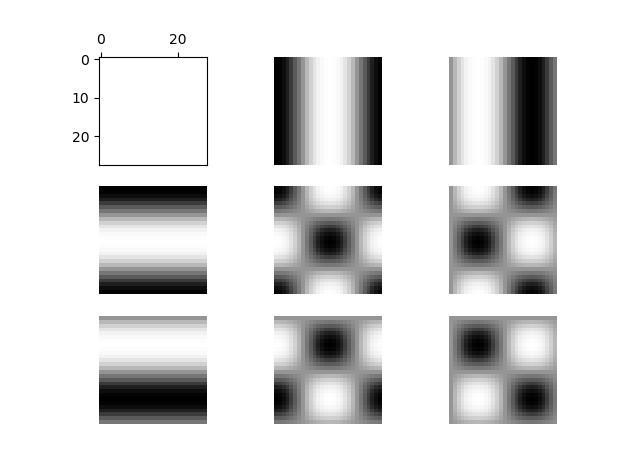
\includegraphics[scale=0.6]{assets/fft-basis}
  \caption{Premiers éléments de la base de Fourier.}
  \label{fig:freq-basis}
\end{figure}

La figure \ref{fig:fft-image-reconstruction} montre la reconstruction d'une 
image en ajoutant progressivement des fréquences.
La figure se lit de gauche à droite et de haut en bas. 
L'image numéro $i$ est reconstruite à partir de tous les coefficients 
d'ordre $p,q < i$ soit $i^2$ coefficients.

\begin{figure}[h]
  \centering
  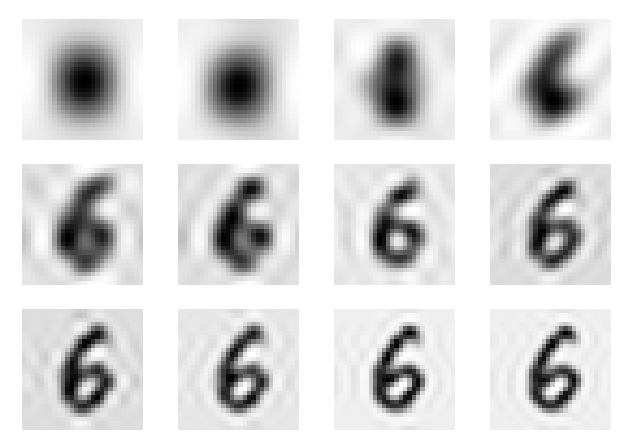
\includegraphics[scale=0.6]{assets/fft-image-num62-reconstruction}
  \caption{Reconstruction d'un $6$.}
  \label{fig:fft-image-reconstruction}
\end{figure}


Dans ce qui suit, on se propose d'expliquer les calculs effectués 
par la fonction \tcode{rfft}.

\renewcommand{\Re}{\operatorname{Re}}
\renewcommand{\Im}{\operatorname{Im}}
\let\conjugatet\overline

Soit $x = (x_0, \cdots, x_{2n-1})$ un vecteur réel de taille $2n$.

On définie la transformée de Fourier discrète de $x$ par un vecteur 
$y$ de même taille dont les composantes sont:
\[
y_j = \sum_{k = 0}^{2n-1} x_k \exp\left(-\frac{2ijk\pi}{2n}\right)
\]

On remarque que $y_j = \operatorname{Conj} y_{2n-j}$. 
Ainsi, seules les valeurs $y_j$ pour $j \leq n$ sont utiles.
De plus, pour $j = n$, on obtient $y_n = \operatorname{Conj} y_{n}$, 
donc la partie imaginaire de $y_n$ est nulle.
Enfin, $y_0$ est un réel.
Ainsi, on peut encoder toute l'information contenue 
dans les $y_j$ pour $j$ de $0$ à $2n-1$ dans de vecteur réel 
$f(x)$ de taille $2n$ définit ci-après.
\[
f(x) = 
\begin{pmatrix}
  y_0 \\
  \Re(y_1) \\
  \Im(y_1) \\
  \vdots \\
  \Re(y_{n-1}) \\
  \Im(y_{n-1}) \\
  \Re(y_n)
\end{pmatrix}
\]

Il est possible de reconstruire $x$ à partir de sa transformée.

\begin{align*}
x^{*}_j &= \frac{1}{2n} \sum_{k=0}^{2n-1} y_k \exp\left( \frac{2ijk\pi}{2n} \right)  \\
        &= \frac{1}{2n} \sum_{k=0}^{2n-1} \sum_{l = 0}^{2n-1} x_l \exp\left(-\frac{2ikl\pi}{2n}\right) \exp\left( \frac{2ijk\pi}{2n} \right) \\
		&= \frac{1}{2n} \sum_{l=0}^{2n-1} \sum_{k = 0}^{2n-1} x_l \exp\left(\frac{2ik(j-l)\pi}{2n}\right) 
\end{align*}

Pour $l = j$, les termes de la seconde somme valent tous $x_l$ et il y en a 
$2n$, on se retrouve donc avec $2n x_l$. \\
Pour $l \neq j$, on a la somme suivante:
\[
x_l \sum_{k = 0}^{2n-1} \exp\left(\frac{2i(j-l)\pi}{2n}\right)^k 
\]
qui est une somme géométrique valant
\[
x_l \times \frac{1-\exp\left(\frac{2i(j-l)\pi}{2n}\right)^{2n}}{1-\exp\left(\frac{2i(j-l)\pi}{2n}\right)} = 0
\]
(que l'on peut également voir comme une somme des racines $2n$-ème de l'unité)

Au final, $x^{*}_j = x_j$.

Une autre écriture de $x^{*}_j$, que l'on utilisera en pratique, est donnée par:

\[
x^{*}_j = \frac{1}{2n} \left[ \sum_{k=1}^{n-1} \left[ y_k \exp\left( \frac{2ijk\pi}{2n} \right) 
          + \overline{y_k} \exp\left(-\frac{2ijk\pi}{2n} \right) \right]
		  + y_0 + (-1)^{j} y_n \right]
\]


Considérons maintenant une matrice $X$ carrée d'ordre $2n$. 
De la même manière que l'on avait vectorisé les fonctions 
d'activation dans la partie concernant les réseaux de neurones, 
on peut vectoriser $f$ et l'appliquer à la matrice $X$. 
On définit donc $f(X)$ comme la matrice dont les colonnes sont 
les images des colonnes de $X$ par $f$.

Le passage d'une image $X$ de dimensions paires dans le domaine 
de Fourier se fait en appliquant la transformée une fois sur les 
colonnes puis une fois sur les lignes. 
La fonction \tcode{rfft} de \tcode{scipy} calcule $f$.
\[
Y = f(f(X)^T)^T
\]
